\hypertarget{t__smat_8c}{
\section{t\_\-smat.c File Reference}
\label{t__smat_8c}\index{t_smat.c@{t\_\-smat.c}}
}


{\tt \#include $<$stdio.h$>$}\par
{\tt \#include $<$stdlib.h$>$}\par
{\tt \#include $<$time.h$>$}\par
{\tt \#include \char`\"{}test-harness.h\char`\"{}}\par
{\tt \#include \char`\"{}dbprim.h\char`\"{}}\par
{\tt \#include \char`\"{}dbprim\_\-int.h\char`\"{}}\par


Include dependency graph for t\_\-smat.c:\begin{figure}[H]
\begin{center}
\leavevmode
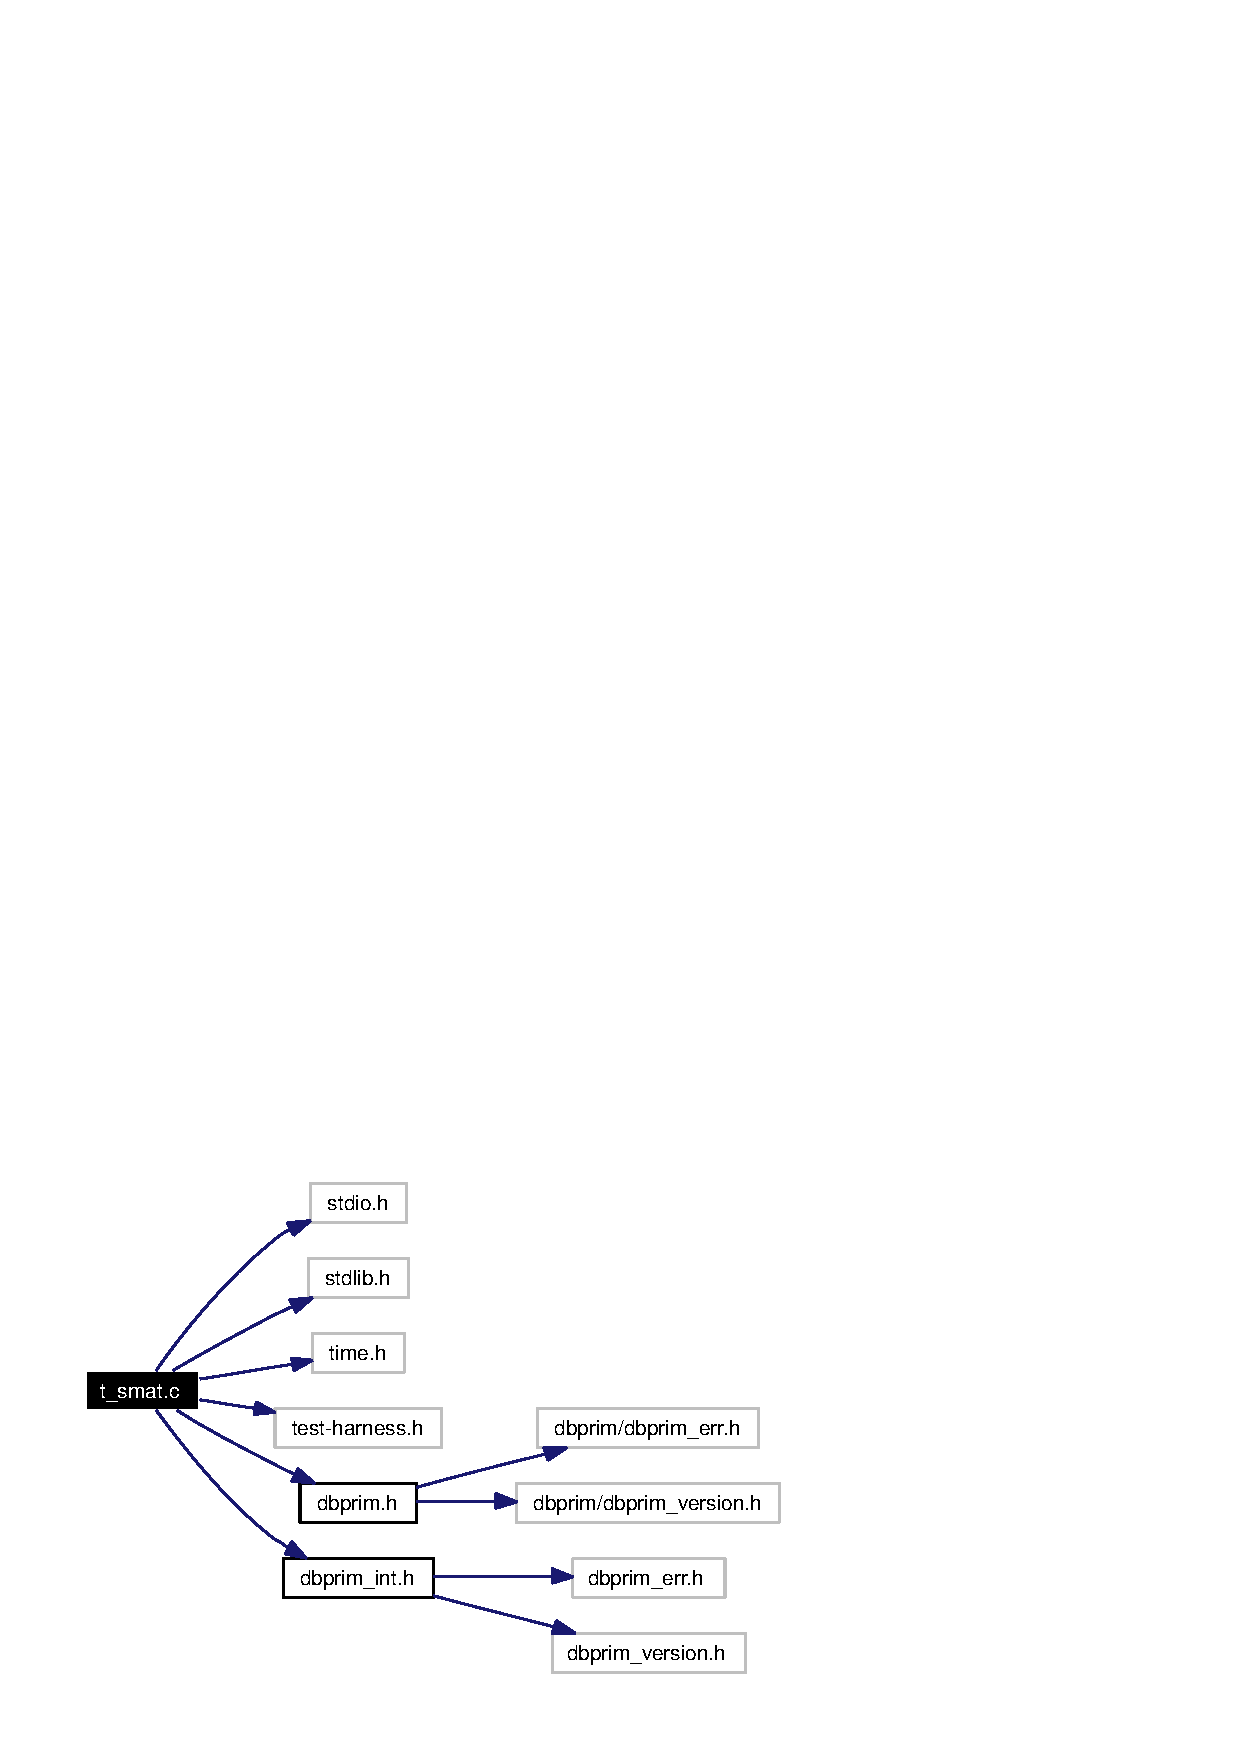
\includegraphics[width=189pt]{t__smat_8c__incl}
\end{center}
\end{figure}
\subsection*{Data Structures}
\begin{CompactItemize}
\item 
struct \hyperlink{structassoc__s}{assoc\_\-s}
\end{CompactItemize}
\subsection*{Defines}
\begin{CompactItemize}
\item 
\#define \hyperlink{t__smat_8c_a0}{SMAT\_\-HEAD\_\-CNT}
\item 
\#define \hyperlink{t__smat_8c_a1}{SMAT\_\-HEAD\_\-MASK}
\item 
\#define \hyperlink{t__smat_8c_a2}{SMAT\_\-ASSOC\_\-CNT}
\item 
\#define \hyperlink{t__smat_8c_a3}{set\_\-assoc}(ass, row, column)
\item 
\#define \hyperlink{t__smat_8c_a4}{clr\_\-assoc}(ass, row, column)
\item 
\#define \hyperlink{t__smat_8c_a5}{chk\_\-assoc}(ass, row, column)
\end{CompactItemize}
\subsection*{Functions}
\begin{CompactItemize}
\item 
static void \hyperlink{t__smat_8c_a9}{set\_\-ones} (struct \hyperlink{structassoc__s}{assoc\_\-s} $\ast$assoc)
\item 
static void \hyperlink{t__smat_8c_a10}{set\_\-zeros} (struct \hyperlink{structassoc__s}{assoc\_\-s} $\ast$assoc)
\item 
static int \hyperlink{t__smat_8c_a11}{check\_\-zeros} (struct \hyperlink{structassoc__s}{assoc\_\-s} $\ast$assoc)
\item 
int \hyperlink{t__smat_8c_a12}{main} (int argc, char $\ast$$\ast$argv)
\end{CompactItemize}
\subsection*{Variables}
\begin{CompactItemize}
\item 
static \hyperlink{struct__smat__head__s}{smat\_\-head\_\-t} \hyperlink{t__smat_8c_a6}{rows} \mbox{[}SMAT\_\-HEAD\_\-CNT\mbox{]}
\item 
static \hyperlink{struct__smat__head__s}{smat\_\-head\_\-t} \hyperlink{t__smat_8c_a7}{columns} \mbox{[}SMAT\_\-HEAD\_\-CNT\mbox{]}
\item 
static struct \hyperlink{structassoc__s}{assoc\_\-s} \hyperlink{t__smat_8c_a8}{associations}
\end{CompactItemize}


\subsection{Define Documentation}
\hypertarget{t__smat_8c_a5}{
\index{t_smat.c@{t\_\-smat.c}!chk_assoc@{chk\_\-assoc}}
\index{chk_assoc@{chk\_\-assoc}!t_smat.c@{t\_\-smat.c}}
\subsubsection[chk\_\-assoc]{\setlength{\rightskip}{0pt plus 5cm}\#define chk\_\-assoc(ass, row, column)}}
\label{t__smat_8c_a5}




Definition at line 88 of file t\_\-smat.c.

Referenced by main().\hypertarget{t__smat_8c_a4}{
\index{t_smat.c@{t\_\-smat.c}!clr_assoc@{clr\_\-assoc}}
\index{clr_assoc@{clr\_\-assoc}!t_smat.c@{t\_\-smat.c}}
\subsubsection[clr\_\-assoc]{\setlength{\rightskip}{0pt plus 5cm}\#define clr\_\-assoc(ass, row, column)}}
\label{t__smat_8c_a4}




Definition at line 86 of file t\_\-smat.c.

Referenced by main().\hypertarget{t__smat_8c_a3}{
\index{t_smat.c@{t\_\-smat.c}!set_assoc@{set\_\-assoc}}
\index{set_assoc@{set\_\-assoc}!t_smat.c@{t\_\-smat.c}}
\subsubsection[set\_\-assoc]{\setlength{\rightskip}{0pt plus 5cm}\#define set\_\-assoc(ass, row, column)}}
\label{t__smat_8c_a3}




Definition at line 84 of file t\_\-smat.c.

Referenced by main().\hypertarget{t__smat_8c_a2}{
\index{t_smat.c@{t\_\-smat.c}!SMAT_ASSOC_CNT@{SMAT\_\-ASSOC\_\-CNT}}
\index{SMAT_ASSOC_CNT@{SMAT\_\-ASSOC\_\-CNT}!t_smat.c@{t\_\-smat.c}}
\subsubsection[SMAT\_\-ASSOC\_\-CNT]{\setlength{\rightskip}{0pt plus 5cm}\#define SMAT\_\-ASSOC\_\-CNT}}
\label{t__smat_8c_a2}




Definition at line 48 of file t\_\-smat.c.

Referenced by main().\hypertarget{t__smat_8c_a0}{
\index{t_smat.c@{t\_\-smat.c}!SMAT_HEAD_CNT@{SMAT\_\-HEAD\_\-CNT}}
\index{SMAT_HEAD_CNT@{SMAT\_\-HEAD\_\-CNT}!t_smat.c@{t\_\-smat.c}}
\subsubsection[SMAT\_\-HEAD\_\-CNT]{\setlength{\rightskip}{0pt plus 5cm}\#define SMAT\_\-HEAD\_\-CNT}}
\label{t__smat_8c_a0}




Definition at line 34 of file t\_\-smat.c.

Referenced by check\_\-zeros(), main(), set\_\-ones(), and set\_\-zeros().\hypertarget{t__smat_8c_a1}{
\index{t_smat.c@{t\_\-smat.c}!SMAT_HEAD_MASK@{SMAT\_\-HEAD\_\-MASK}}
\index{SMAT_HEAD_MASK@{SMAT\_\-HEAD\_\-MASK}!t_smat.c@{t\_\-smat.c}}
\subsubsection[SMAT\_\-HEAD\_\-MASK]{\setlength{\rightskip}{0pt plus 5cm}\#define SMAT\_\-HEAD\_\-MASK}}
\label{t__smat_8c_a1}




Definition at line 40 of file t\_\-smat.c.

Referenced by set\_\-ones().

\subsection{Function Documentation}
\hypertarget{t__smat_8c_a11}{
\index{t_smat.c@{t\_\-smat.c}!check_zeros@{check\_\-zeros}}
\index{check_zeros@{check\_\-zeros}!t_smat.c@{t\_\-smat.c}}
\subsubsection[check\_\-zeros]{\setlength{\rightskip}{0pt plus 5cm}static int check\_\-zeros (struct \hyperlink{structassoc__s}{assoc\_\-s} $\ast$ {\em assoc})\hspace{0.3cm}{\tt  \mbox{[}static\mbox{]}}}}
\label{t__smat_8c_a11}




Definition at line 72 of file t\_\-smat.c.

References assoc\_\-s::assoc, and SMAT\_\-HEAD\_\-CNT.

Referenced by main().\hypertarget{t__smat_8c_a12}{
\index{t_smat.c@{t\_\-smat.c}!main@{main}}
\index{main@{main}!t_smat.c@{t\_\-smat.c}}
\subsubsection[main]{\setlength{\rightskip}{0pt plus 5cm}int main (int {\em argc}, char $\ast$$\ast$ {\em argv})}}
\label{t__smat_8c_a12}




Definition at line 92 of file t\_\-smat.c.

References associations, check\_\-zeros(), chk\_\-assoc, clr\_\-assoc, LINK\_\-LOC\_\-HEAD, se\_\-object, set\_\-assoc, set\_\-ones(), set\_\-zeros(), sh\_\-init(), SMAT\_\-ASSOC\_\-CNT, SMAT\_\-HEAD\_\-CNT, SMAT\_\-LOC\_\-FIRST, SMAT\_\-LOC\_\-SECOND, st\_\-add(), st\_\-count, st\_\-find(), st\_\-init(), st\_\-modulus, and st\_\-remove().

Here is the call graph for this function:\begin{figure}[H]
\begin{center}
\leavevmode
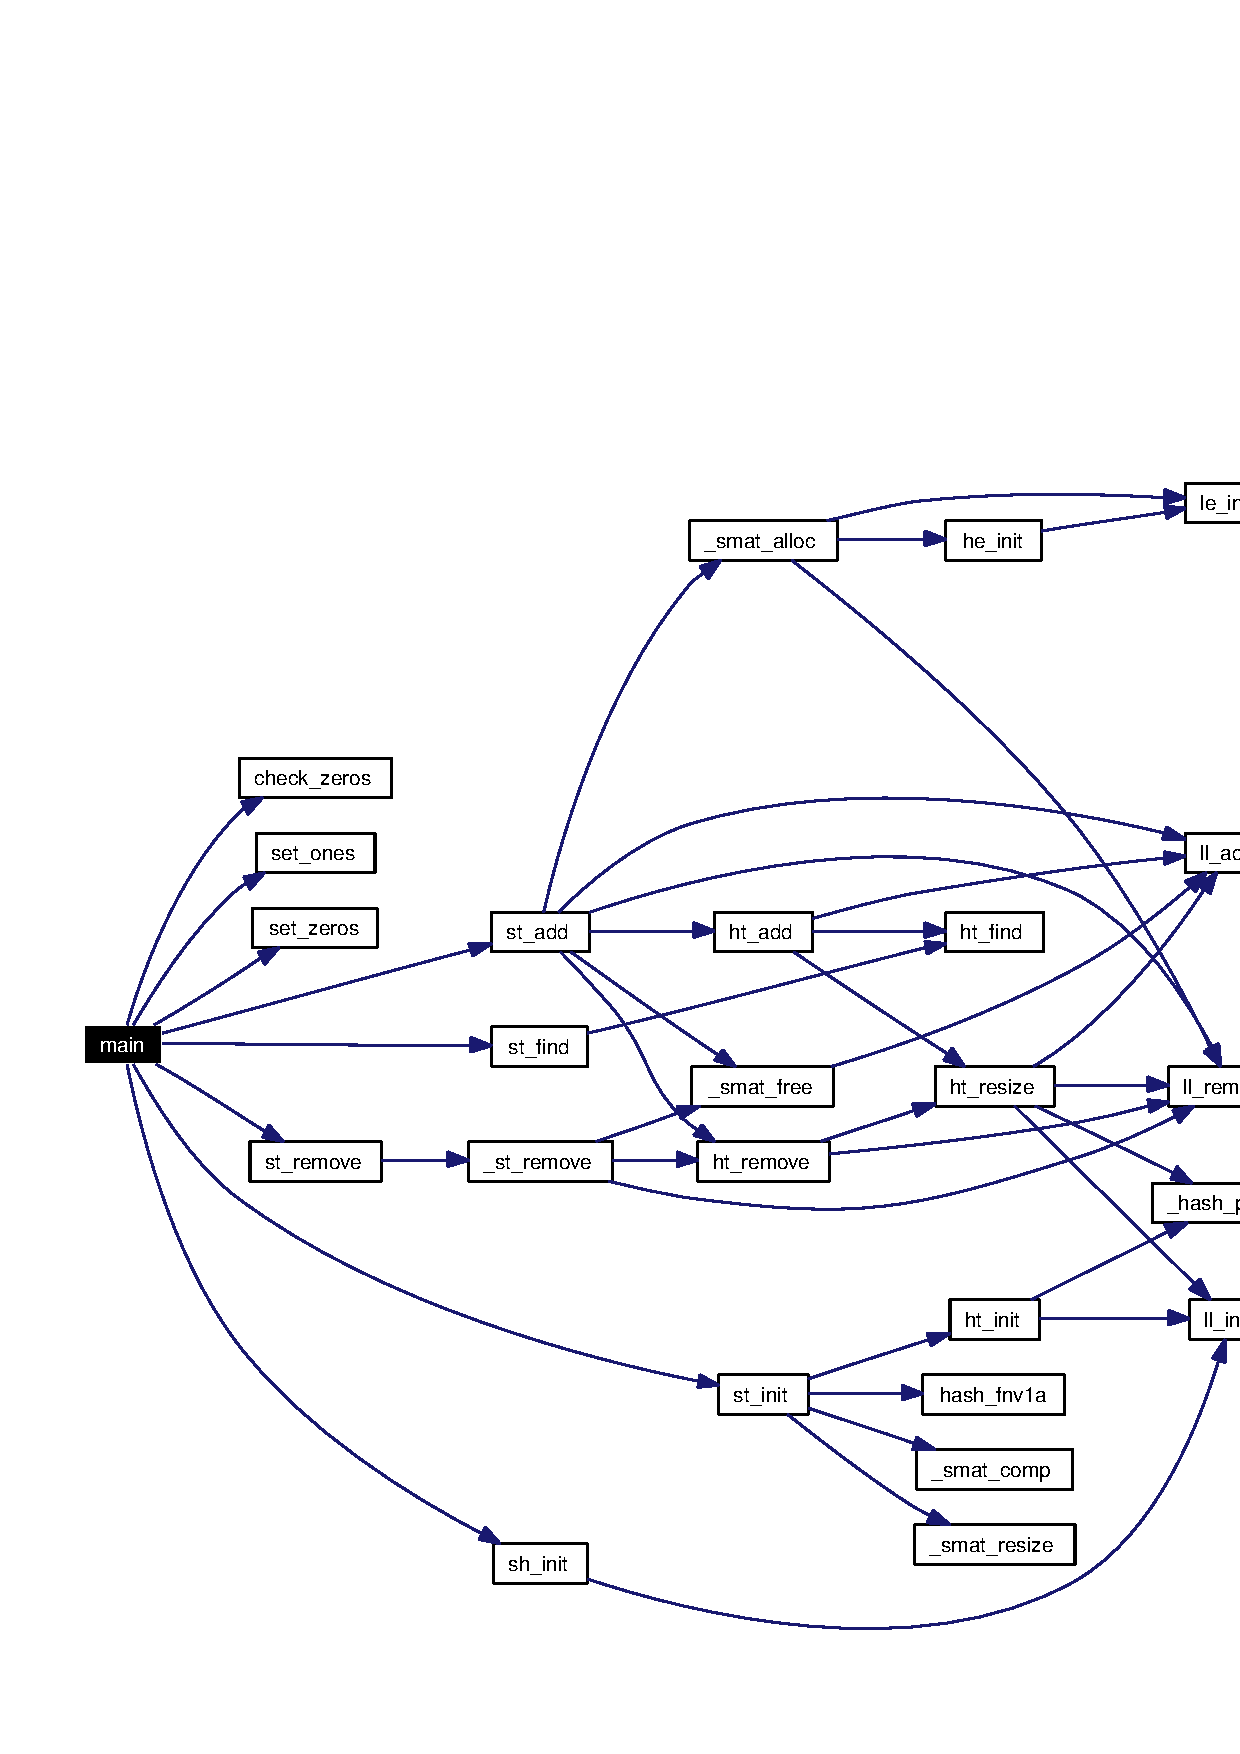
\includegraphics[width=316pt]{t__smat_8c_a12_cgraph}
\end{center}
\end{figure}
\hypertarget{t__smat_8c_a9}{
\index{t_smat.c@{t\_\-smat.c}!set_ones@{set\_\-ones}}
\index{set_ones@{set\_\-ones}!t_smat.c@{t\_\-smat.c}}
\subsubsection[set\_\-ones]{\setlength{\rightskip}{0pt plus 5cm}static void set\_\-ones (struct \hyperlink{structassoc__s}{assoc\_\-s} $\ast$ {\em assoc})\hspace{0.3cm}{\tt  \mbox{[}static\mbox{]}}}}
\label{t__smat_8c_a9}




Definition at line 52 of file t\_\-smat.c.

References assoc\_\-s::assoc, SMAT\_\-HEAD\_\-CNT, and SMAT\_\-HEAD\_\-MASK.

Referenced by main().\hypertarget{t__smat_8c_a10}{
\index{t_smat.c@{t\_\-smat.c}!set_zeros@{set\_\-zeros}}
\index{set_zeros@{set\_\-zeros}!t_smat.c@{t\_\-smat.c}}
\subsubsection[set\_\-zeros]{\setlength{\rightskip}{0pt plus 5cm}static void set\_\-zeros (struct \hyperlink{structassoc__s}{assoc\_\-s} $\ast$ {\em assoc})\hspace{0.3cm}{\tt  \mbox{[}static\mbox{]}}}}
\label{t__smat_8c_a10}




Definition at line 62 of file t\_\-smat.c.

References assoc\_\-s::assoc, and SMAT\_\-HEAD\_\-CNT.

Referenced by main().

\subsection{Variable Documentation}
\hypertarget{t__smat_8c_a8}{
\index{t_smat.c@{t\_\-smat.c}!associations@{associations}}
\index{associations@{associations}!t_smat.c@{t\_\-smat.c}}
\subsubsection[associations]{\setlength{\rightskip}{0pt plus 5cm}struct \hyperlink{structassoc__s}{assoc\_\-s}  \hyperlink{t__smat_8c_a8}{associations}\hspace{0.3cm}{\tt  \mbox{[}static\mbox{]}}}}
\label{t__smat_8c_a8}




Referenced by main().\hypertarget{t__smat_8c_a7}{
\index{t_smat.c@{t\_\-smat.c}!columns@{columns}}
\index{columns@{columns}!t_smat.c@{t\_\-smat.c}}
\subsubsection[columns]{\setlength{\rightskip}{0pt plus 5cm}\hyperlink{struct__smat__head__s}{smat\_\-head\_\-t} \hyperlink{t__smat_8c_a7}{columns}\mbox{[}SMAT\_\-HEAD\_\-CNT\mbox{]}\hspace{0.3cm}{\tt  \mbox{[}static\mbox{]}}}}
\label{t__smat_8c_a7}




Definition at line 43 of file t\_\-smat.c.\hypertarget{t__smat_8c_a6}{
\index{t_smat.c@{t\_\-smat.c}!rows@{rows}}
\index{rows@{rows}!t_smat.c@{t\_\-smat.c}}
\subsubsection[rows]{\setlength{\rightskip}{0pt plus 5cm}\hyperlink{struct__smat__head__s}{smat\_\-head\_\-t} \hyperlink{t__smat_8c_a6}{rows}\mbox{[}SMAT\_\-HEAD\_\-CNT\mbox{]}\hspace{0.3cm}{\tt  \mbox{[}static\mbox{]}}}}
\label{t__smat_8c_a6}




Definition at line 42 of file t\_\-smat.c.